
\documentclass[a4paper,UTF8]{article}
\usepackage{ctex}
\usepackage[margin=1.25in]{geometry}
\usepackage{color}
\usepackage{graphicx}
\usepackage{amssymb}
\usepackage{amsmath}
\usepackage{amsthm}
\usepackage{soul, color, xcolor}
\usepackage{bm}
\usepackage{tcolorbox}
\usepackage{hyperref}
\numberwithin{equation}{section}
%\usepackage[thmmarks, amsmath, thref]{ntheorem}
\theoremstyle{definition}
\newtheorem*{solution}{Solution}
\newtheorem*{prove}{Proof}
\usepackage{multirow}
\usepackage{diagbox}
\usepackage{float}

\def \X {\mathbf{X}}
\def \A {\mathbf{A}}
\def \w {\hat{\boldsymbol{w}}}
\def \y {\mathbf{y}}
\def \x {\mathbf{x}}
\def \z {\mathbf{z}}
\def \hy {\widehat{y}}
\def \by {\Bar{y}}
\def \H {\mathbf{H}}
\def \I {\mathbf{I}}
\setlength{\parindent}{0pt}
%--

%--
\begin{document}
\title{机器学习导论\ 习题一}
\author{201840009, 田永上, \href{mailto:邮箱}{201840009@smail.nju.edu.cn}}
\maketitle
\section*{作业提交注意事项}
\begin{tcolorbox}
	\begin{enumerate}
		\item[1.] 请在LaTeX模板中第一页填写个人的学号、姓名、邮箱;
		\item[2.] 本次作业需提交作答后的该 pdf 文件、编程题代码(.py文件); {\color{red}\textbf{请将二者打包为~.zip 文件上传}}. 注意命名规则, 三个文件均命名为 “学号\_姓名” + “.后缀” (例如 211300001\_张三” + “.pdf”、“.py”、“.zip”);
		\item[3.] 若多次提交作业, 则在命名~.zip 文件时加上版本号, 例如 211300001\_张三\_v1.zip” (批改时以版本号最高的文件为准);
		\item[4.] 本次作业提交截止时间为 {\color{red}\textbf{ 3 月 29 日23:59:59}}. 未按照要求提交作业, 提交作业格式不正确, {\color{red}\textbf{作业命名不规范}}, 将会被扣除部分作业分数; 除特殊原因 (如因病缓交, 需出示医院假条) 逾期未交作业, 本次作业记 0 分; {\color{red}\textbf{如发现抄袭, 抄袭和被抄袭双方成绩全部取消}};
		\item[5.] 本次作业提交地址为 \href{https://box.nju.edu.cn/u/d/008080744a60484ea526/}{here}, 请大家预留时间提前上交, 以防在临近截止日期时, 因网络等原因无法按时提交作业.
	\end{enumerate}
\end{tcolorbox}
\newpage


\section{[15pts] Derivatives of Matrices}
 有 $\alpha \in \mathbb{R}$, $\y\in \mathbb{R}^{m×1}$, $\x\in \mathbb{R}^{n×1}$, 试完成下题, 并给出计算过程.
\begin{enumerate}
	\item[(1)] \textbf{[4pts]} 此问中假设 $\A\in \mathbb{R}^{n×n}$, 且 $\alpha=\x^\top\A\x$, 试求 $\frac{\partial \alpha}{\partial \x}$.
	\item[(2)] \textbf{[5pts]} 此问中假设 $\A\in \mathbb{R}^{m×n}$, 且 $\alpha=\y^\top\A\x$, 同时 $\y$、$\x$ 为 $\z$ 的函数, 试求 $\frac{\partial \alpha}{\partial \z}$.
	\item[(3)] \textbf{[6pts]} 此问中假设 $\A\in \mathbb{R}^{n×n}$ 且 $\A$ 可逆, $\A$ 为 $\alpha$ 的函数同时 $\frac{\partial \A}{\partial \alpha}$ 已知. 试求 $\frac{\partial \A^{-1}}{\partial \alpha}$.
\end{enumerate}
(提示: 可以参考 \href{https://www.math.uwaterloo.ca/~hwolkowi/matrixcookbook.pdf}{The Matrix Cookbook}.)

\begin{solution}
	~\\
	(1)$\alpha = \sum_{i=1}^{n} x_i \sum_{j=1}^{n} a_{ij}x_{j}$\\
	对于$x_k$,$\frac{\partial \alpha}{\partial x_k}=\sum_{i=1}^{n} (a_{ik}+a_{ki})x_k$\\
	所以,$\frac{\partial \alpha}{\partial x}=(A+A^T)x$\\
	(2)$\frac{\partial \alpha}{\partial \z}=\frac{\partial \alpha}{\partial \x}\frac{\partial \x}{\partial \z}+\frac{\partial \alpha}{\partial \y}\frac{\partial \y}{\partial \z}=(y^TA)^T \frac{\partial \x}{\partial \z}+(Ax)\frac{\partial \y}{\partial \z}=(A^T y) \frac{\partial \x}{\partial \z}+(Ax)\frac{\partial \y}{\partial \z}$\\
	(3)已知$I=AA^-1$\\
	那么,$\frac{\partial I}{\partial \alpha}=\frac{\partial A}{\partial \alpha}A^{-1}+\frac{\partial A^{-1}}{\partial \alpha} A=0$\\
	所以,$\frac{\partial A}{\partial \alpha}A^{-1}=-\frac{\partial A^{-1}}{\partial \alpha} A \quad \implies \frac{\partial A^{-1}}{\partial \alpha}=-A^{-1} \frac{\partial A}{\partial \alpha} A^{-1}$
\end{solution}




\newpage
\section{[15pts] Performance Measure}
 性能度量是衡量模型泛化能力的评价标准, 在对比不同模型的能力时, 使用不同的性能度量往往会导致不同的评判结果.
请仔细阅读《机器学习》第二章 2.3.3 节. 在书中, 我们学习并计算了模型的二分类性能度量. 下面我们给出一个多分类 (四分类) 的例子, 请根据学习器的具体表现, 回答如下问题.
\begin{table}[ht]
	\centering
	\caption{类别的真实标记与预测}
	\label{tab:samples1}
	\begin{tabular}{|l|l|l|l|l|}
		\hline
	\diagbox{真实类别}{预测类别}   & 第一类 & 第二类 & 第三类 & 第四类 \\ \hline
	第一类 & 7   & 2   & 1   & 0   \\ \hline
	第二类 & 0   & 9   & 0   & 1   \\ \hline
	第三类 & 1   & 0   & 8   & 1   \\ \hline
	第四类 & 1   & 2   & 1   & 6   \\ \hline
	\end{tabular}
\end{table}
\begin{enumerate}
	\item[(1)] \textbf{[5pts]}  如表~\ref{tab:samples1} 所示, 请计算该学习器的错误率及精度.
	\item[(2)] \textbf{[5pts]}  请分别计算宏查准率, 宏查全率, 微查准率, 微查全率, 并两两比较大小.
	\item[(3)] \textbf{[5pts]}  分别使用宏查准率, 宏查全率, 微查准率, 微查全率计算宏$F1$度量, 微$F1$度量, 并比较大小.

\end{enumerate}


\begin{solution}
	~\\
	(1)类比二元形式,进行定义$F_i P_j$实际i类预测为j类,$FP_i$表示非i类预测为i类,实际上是一列中错误的个数\\
	$errorrate=\frac{\sum_{i=1}^{4} FP_i}{40}=0.25$\\
	$accuracy=1-errorrate=0.75$\\
	(2)先算$P_i=\frac{TP_i}{TP_i+FP_i}$\\
	$P_1=\frac{7}{9},P_2=\frac{9}{13},P_3=\frac{4}{5},P_4=\frac{3}{4}$\\
	宏查准率=$\frac{1}{4} (P_1+P_2+P_3+P_4)=\frac{7067}{9360}=0.755$\\
	再算$R_i=\frac{TP_i}{TP_i+FN_i}$\\
	$R_1=0.7,R_2=0.9,R_3=0.8,R_4=0.6$\\
	宏查全率=$\frac{1}{4} (R_1+R_2+R_3+R_4)=0.75$\\
	$\overline{TP}=7.5,\overline{FP}=2.5,\overline{FN}=2.5$\\
	微查准率=$\frac{\overline{TP}}{\overline{TP}+\overline{FP}}=0.75$\\
	微查全率=$\frac{\overline{TP}}{\overline{TP}+\overline{FN}}=0.75$\\
	(3)宏F1度量=$\frac{2*macro-P*macro-R}{macro-P+macro-R}=0.7525$\\
	微F1度量=$\frac{2*micro-P*micro-R}{micro-P+micro-R}=0.75$\\
\end{solution}

\newpage

\section{[15pts] ROC \& AUC}
 ROC 曲线与其对应的 AUC 值可以反应分类器在 “一般情况下” 泛化性能的好坏. 请仔细阅读《机器学习》第二章 2.3.3 节,并完成本题.
\begin{table}[ht]
	\centering
	\caption{样例的真实标记与预测}
	\begin{tabular}{c|ccccccccc}
		\hline 样例 & $x_1$ & $x_2$ & $x_3$ & $x_4$ & $x_5$ & $x_6$ & $x_7$ & $x_8$ & $x_9$ \\
		\hline 标记 & 0 & 1 & 0 & 1 & 0 & 0 & 1 & 1 & 0 \\
		\hline 分类器输出值 & 0.4 & 0.9 & 0.7 & 0.4 & 0.2 & 0.8 & 0.8 & 0.6 & 0.5 \\
		\hline
	\end{tabular}
	\label{tab:samples}
\end{table} 
\begin{enumerate}
    \item[(1)] \textbf{[5pts]}  如表~\ref{tab:samples} 所示, 第二行为样例对应的真实标记, 第三行为某分类器对样例的预测结果. 请根据上述结果, 绘制分类器在该样例集合上的 ROC 曲线, 并写出绘图中使用到的节点 (在坐标系中的) 坐标及其对应的阈值与样例编号.
    \item[(2)] \textbf{[3pts]}  根据上题中的 ROC 曲线, 计算其对应的 AUC 值(请给出具体的计算步骤).
    \item[(3)] \textbf{[7pts]}  结合前两问使用的例子(可以借助图片示意), 试证明对有限样例成立:
    \begin{equation}
        \label{eq:auc}
            \text{AUC} = \frac{1}{m^+m^-}\sum_{x^+\in D^+}\sum_{x^-\in D^-}\left(\mathbb{I}\left\{f(x^+) > f(x^-)\right\}+\frac{1}{2}\mathbb{I}\left\{f(x^+)=f(x^-)\right\}\right).
    \end{equation}    
\end{enumerate}


\begin{solution}
	~\\
	(1)坐标如下:[(0, 0), (0.0, 0.25), (0.2, 0.5), (0.4, 0.5), (0.4, 0.75), (0.6, 0.75), (0.8, 1.0), (1.0, 1.0)],ROC曲线如下:
	\begin{figure}[htbp]
		\centering
		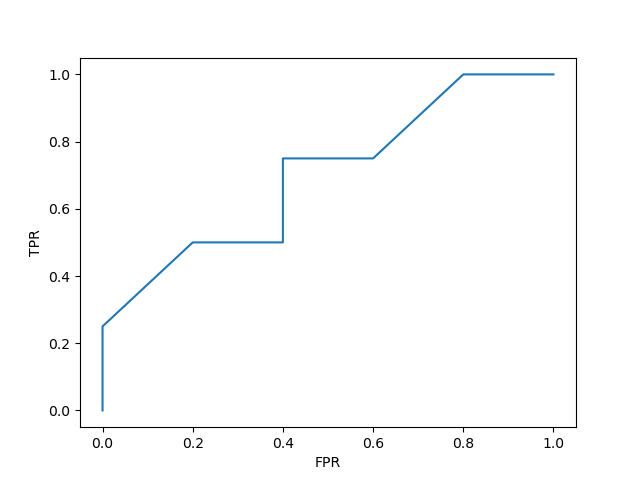
\includegraphics[scale=0.8]{1.jpg}
	\end{figure}\\
	~\\
	(2)坐标中每一项元素为$(x_i,y_i)$\\
	那么AUC=$\frac{1}{2} \sum_{i=1}^{7} (x_{i+1}-x_i)(y_{i+1}-y_i)=0.075+0.1+0.15+0.175+0.2=0.7$\\
	(3)首先对于$l_{rank}$进行简单变形\\
	$$l_{rank}=\sum_{x^+\in D^+} \frac{1}{2} \frac{1}{m^+} \sum_{x^-\in D^-}\left(\frac{2}{m^-}\mathbb{I}\left\{f(x^+) > f(x^-)\right\}+\frac{1}{m^-}\mathbb{I}\left\{f(x^+)=f(x^-)\right\}\right)$$\\
	考虑新增真正例后的变化,记当前标记点为$(x,y)$,那么下一个标记点为$(x,y+\frac{1}{m^+})$
	考虑$l_{rank}$的含义,可以理解为ROC曲线和y轴所围城的面积,在绘制ROC曲线的过程中,如果新增点,那么用梯形面积的公式来计算$l_{rank}$新增加的面积,那么梯形的高为$\frac{1}{m^+}$\\
	再看梯形的底,在绘制的过程中每增加一个假正例会在x方向增加一个步长$\frac{1}{m^-}$,那么就看当前阈值为$f(x^+)$时假正例的个数\\
	较短的一个底的长度为$\sum_{x^-\in D^-} (\frac{1}{m^-}\mathbb{I}\left\{f(x^+) > f(x^-)\right\}$\\
	对于较长的一个底的长度为$\sum_{x^-\in D^-}\left(\frac{1}{m^-}\mathbb{I}\left\{f(x^+) > f(x^-)\right\}+\frac{1}{m^-}\mathbb{I}\left\{f(x^+)=f(x^-)\right\}\right)$\\
	那么新增一个真正例后,增加的梯形的面积为$$\frac{1}{2} \frac{1}{m^+} \sum_{x^-\in D^-}\left(\frac{2}{m^-}\mathbb{I}\left\{f(x^+) > f(x^-)\right\}+\frac{1}{m^-}\mathbb{I}\left\{f(x^+)=f(x^-)\right\}\right)$$\\
	$l_{rank}$的计算过程可以视为是不断新增真正例,不断增加面积的过程\\
	所以$$l_{rank}=\sum_{x^+\in D^+} \frac{1}{2} \frac{1}{m^+} \sum_{x^-\in D^-}\left(\frac{2}{m^-}\mathbb{I}\left\{f(x^+) > f(x^-)\right\}+\frac{1}{m^-}\mathbb{I}\left\{f(x^+)=f(x^-)\right\}\right)$$得证\\
	这个形式和原题目中形式等价,原题得证
\end{solution}
\newpage




\section{[20pts] Linear Regression}
 线性回归模型是一类常见的机器学习方法, 其基础形式与变体常应用在回归任务中. 根据《机器学习》第三章 3.2 节中的定义, 可以将收集到的 $d$ 维数据及其标签如下表示: 

\[
\X=\left(\begin{array}{ccccc}
x_{11} & x_{12} & \ldots & x_{1 d} & 1 \\
x_{21} & x_{22} & \ldots & x_{2 d} & 1 \\
\vdots & \vdots & \ddots & \vdots & \vdots \\
x_{m 1} & x_{m 2} & \cdots & x_{m d} & 1
\end{array}\right)
=
\left(\begin{array}{cc}
\x_1^{\top} & 1 \\
\x_2^{\top} & 1 \\
\vdots & \vdots \\
\x_m^{\top} & 1
\end{array}\right)
;\quad \y 
=
\left(\begin{array}{c}
y_1\\
y_2\\
\vdots\\
y_m
\end{array}\right).
\]

将参数项与截距项合在一起, 定义为$\w=
\left(
\boldsymbol{w}^\top; b\right)^\top$. 此时成立 $\hat{\y} = \X\w$.《机器学习》式 (3.11) 给出了最小二乘估计 (Least Square Estimator, LSE) 的闭式解: 
\begin{equation}
    \label{eq:LSE}
    \w_{\textbf{LSE}}^* = \left(\X^\top\X\right)^{-1}\X^\top\y.
\end{equation}
  
\begin{enumerate}
\item[(1)] \textbf{[8pts]} (投影矩阵的性质) 
% 在得到 $\w^*$ 后,可使用 $\mathbf{\hy} = \X \w^*$ 得到样本标记的预测值.
容易验证, 当采用最小二乘估计 $\w_{\textbf{LSE}}^*$ 时, 成立: 
\begin{equation*}
    \mathbf{\hy} = \X \w_{\textbf{LSE}}^* = \X\left(\X^\top\X\right)^{-1}\X^\top\y.
\end{equation*}

记 $\H = \X\left(\X^\top\X\right)^{-1}\X^\top$, 则有 $\mathbf{\hy} = \H\y$. $\H$ 被称为 “Hat Matrix”, 其存在可以从空间的角度, 把 $\mathbf{\hy}$ 看作是 $\y$ 在矩阵 $\H$ 空间中的投影. $\H$ 矩阵有着许多良好的性质.
已知此时 $\X$ 矩阵列满秩, $\I$ 为单位阵, 试求 $\I - \H$ 的全部特征值并注明特征值的重数.
% \begin{center}
% \fcolorbox{gray}{gray!10}{\parbox{.85\linewidth}{背景: 记 $\H = \X\left(\X^\top\X\right)^{-1}\X^\top$,则有$\mathbf{\hy} = \H\y$.\\$\H$ 被称为“Hat Matrix”,其存在可以从空间的角度,把 $\mathbf{\hy}$ 看作是 $\y$ 在矩阵 $\H$ 空间中的投影.$\H$ 矩阵有着许多良好的性质.}}
% \end{center}

(提示: 利用 $\H$ 矩阵的投影性质与对称性.)



\item[(2)] \textbf{[5pts]} (岭回归) 当数据量 $m$ 较小或数据维度 $d$ 较高时, 矩阵 $\X^\top\X$ 可能不满秩, \ref{eq:LSE} 中的取逆操作难以实现. 此时可使用岭回归代替原始回归问题, 其形式如下: 
\begin{equation}
    \label{eq:Ridge}
    \w_{\textbf{Ridge}}^* = \mathop{\arg\min}_{\w} \frac{1}{2}\left(\lVert \y - \X \w \rVert_2^2 +\lambda \lVert \w \rVert_2^2\right).
\end{equation}
试求岭回归问题的闭式解, 并简述其对原问题的改进.

\item[(3)] \textbf{[7pts]} 定义 $\Tilde{\x}_i = \left(\x_i^\top;1\right)^\top$,
$\hy_i = \Tilde{\x}_i^\top \w_{\textbf{LSE}}^*$,
$\by = \frac{1}{m} \sum\limits_{i=1}^m y_i $. 

对线性回归模型进行统计分析时,会涉及如下三个基础定义: 
\begin{equation*}
    \left\{
        \begin{aligned}
        &\text{Total sum of squares (SST): }& &\sum\limits_{i=1}^m\left(y_i-\by\right)^2 \\
        &\text{Regression sum of squares (SSR): }& &\sum\limits_{i=1}^m\left(\hy_i-y_i\right)^2 \\
        &\text{Residual sum of squares (SSE): }& &\sum\limits_{i=1}^m\left(\hy_i-\by\right)^2
        \end{aligned}
    \right.
\end{equation*}

试证明 SST = SSR + SSE. (提示: 使用向量形式可以简化证明步骤.)



\end{enumerate}


\begin{solution}
	~\\
	(1)H具有幂等性,即$H^2=X(X^T X)^{-1}X^T X(X^T X)^{-1}X^T=X (X^T X)^{-1} (X^T X) (X^T X)^{-1} X^T=X (X^T X)^{-1} X^T=H$\\
	那么,$(I-H)^2 y=I-2H+H^2=I-H$也具有幂等性\\
	所以$(I-H)^2 y=(I-H)y=\lambda^2 y=\lambda y$,可得$\lambda=0,1$\\
	0的重数为1,1的重数为n-1,n是矩阵的阶数\\
	(2)记需要最小化的部分为L\\
	$$\frac{\partial L}{\partial w}=-2X^T (y-Xw)+2\lambda w=0$$
	得到$$w_{ridge}=(X^TX+\lambda I)^{-1} X^T y$$\\
	(3)\begin{align*}
		SST=&\sum_{i=1}^{m}(y_i-\hat {y_i}+\hat{y_i}-\overline{y})\\
		=&SSR+SSE+2\sum_{i=1}^{m}(y_i-\hat {y_i})(\hat{y_i}-\overline{y})\\
	\end{align*}
	另外,最优化的结果最小化了SSR,所以还满足下面的条件:\\
	\begin{align*}
		&\frac{\partial SSR}{\partial w}=\frac{\partial \sum_{i=1}^{m}(w^T x_i+b-y_i)^2}{\partial w}=2\sum_{i=1}^{m}x_i(w^T x_i+b-y_i)=\vec{0}\\
		&\frac{\partial SSR}{\partial b}=\frac{\partial \sum_{i=1}^{m}(w^T x_i+b-y_i)^2}{\partial b}=2\sum_{i=1}^{m}(w^T x_i+b-y_i)=\vec{0}\\
		&\sum_{i=1}^{m}(y_i-\hat {y_i})(\hat{y_i}-\overline{y})=\sum_{i=1}^{m}(y_i-\hat {y_i})(w^T x_i+b-\overline{y})\\
		&=\sum_{i=1}^{m}w^T x_i(y_i-\hat {y_i})+\sum_{i=1}^{m}(b-\overline{y})(y_i-\hat {y_i})=0
	\end{align*}
	SST=SSR+SSE得证
\end{solution}

\newpage
\section{[35pts] Logistic Regression in Practice}
对数几率回归 (Logistic Regression, 简称LR) 是实际应用中非常常用的分类学习算法.
\begin{enumerate}
    \item[(1)]  \textbf{[30pts]} 请编程实现二分类的 LR, 要求采用牛顿法进行优化求解. 详细编程题指南请参见链接: \href{https://www.lamda.nju.edu.cn/ML2023Spring/homework/hw1/hw1-code.html}{here}. 请将绘制好的 ROC 曲线放在解答处, 并记录模型的精度与 AUC (保留4位小数).
    \item[(2)]  \textbf{[5pts]} 试简述在对数几率回归中, 相比梯度下降方法, 使用牛顿法的优点和缺点.
\end{enumerate}

\begin{solution}
此处用于写解答 (中英文均可)
~\\
%%%%% use following code to insert the picture %%%%%
% (1) 
% \begin{figure}[H]
% \centering
% \includegraphics[width=0.8\textwidth]{roc.png}\\
% \caption{ROC of test set}
% \label{fig:roc}
% \end{figure}\\
~\\
~\\
~\\
\end{solution}



\end{document}